\documentclass[compacto]{aleph-notas}

\usepackage{aleph-comandos}
\usepackage{enumitem}
\usepackage{parskip}
\usepackage{amssymb}
\usepackage{multicol}
\usepackage{amsmath}
\usepackage{graphicx}
\usepackage{algorithm}
\usepackage[noend]{algpseudocode}
\usepackage{xcolor}
\usepackage{listings}
\graphicspath{ {./img/} }
\setlength\parindent{0pt}

\institucion{Compiladores}
\autor{Maximiliano Onofre Martínez \\422054438}
\tema{Práctica 1}
\fuente{montserrat}
\logouno[6.5cm]{img/fc}

\begin{document}
\encabezado
\begin{ejer}
¿Qué ocurre si en la primera sección se quitan las llaves al nombre de la macro letra?
\end{ejer}
La primera sección le corresponde a las expresiones regulares, las cuales tienen la forma
\texttt{<Expresión Regular>=\{<Acción Léxica>\}}. La acción léxica se ejecuta cada vez que
se encuentra una cadena que coincida con la expresión regular, por lo tanto, si quitamos las llaves en
\texttt{palabra=\{letra\}+}, entonces el programa solo podrá identificar números.

\begin{ejer}
¿Qué ocurre si en la segunda sección se quitan las llaves a las macros?
\end{ejer}

Si quitamos las llaves a las macros en esta sección, entonces tenemos que al ejecutar \texttt{java Lexer
  input.txt}, el resultado es el contenido de la entrada sin analizar,
esto se debe a que estamos declarando las macros pero nunca
las utilizamos (cosa que nos advierte el mismo compilador), por lo que las llaves resultan indispensables.

\begin{ejer}
¿Cómo se escribe un comentario en flex?
\end{ejer}
Flex admite comentarios de estilo C, es decir, cualquier cosa entre '/*' y '*/' se considera un comentario.
\begin{ejer}
¿Qué se guarda en yytext?
\end{ejer}
En yytext se guarda la cadena que pertenece a las expresiones regulares asignadas en las macros,
para que podamos usarla en nuestras funciones auxiliares al momento del análisis léxico.
\begin{ejer}
¿Qué pasa al ejecutar el programa e introducir cadenas de caracteres y de dígitos en el archivo de entrada?
\end{ejer}
Si en el archivo de entrada hay cadenas de caracteres y dígitos, entonces nuestro
programa analizará correctamente su contenido e imprimirá las palabras y los números que compongan dichos elementos.

\begin{ejer}
¿Qué ocurre si introducimos caracteres como ``*'' en el archivo de entrada?
\end{ejer}
Como este carácter no ha sido capturado por ninguna de nuestras reglas,
entonces el analizador léxico no hará más que ignorarlo, es decir, seguirá funcionando salvo con aquellos elementos que no hemos englobado con nuestras expresiones regulares.

\begin{ejer}
Modificar al código anterior en un archivo nuevo, de tal manera que reconozca lo siguiente:
        \begin{itemize}
        \item La expresión regular para los hexadecimales en lenguaje Java.
        \item 5 palabras reservadas del lenguaje Java.
        \item Los identificadores válidos del lenguaje Java, con longitud de a lo más 32 caracteres.
          \item Los espacios en blanco.
        \end{itemize}
\end{ejer}
\begin{figure}[h]
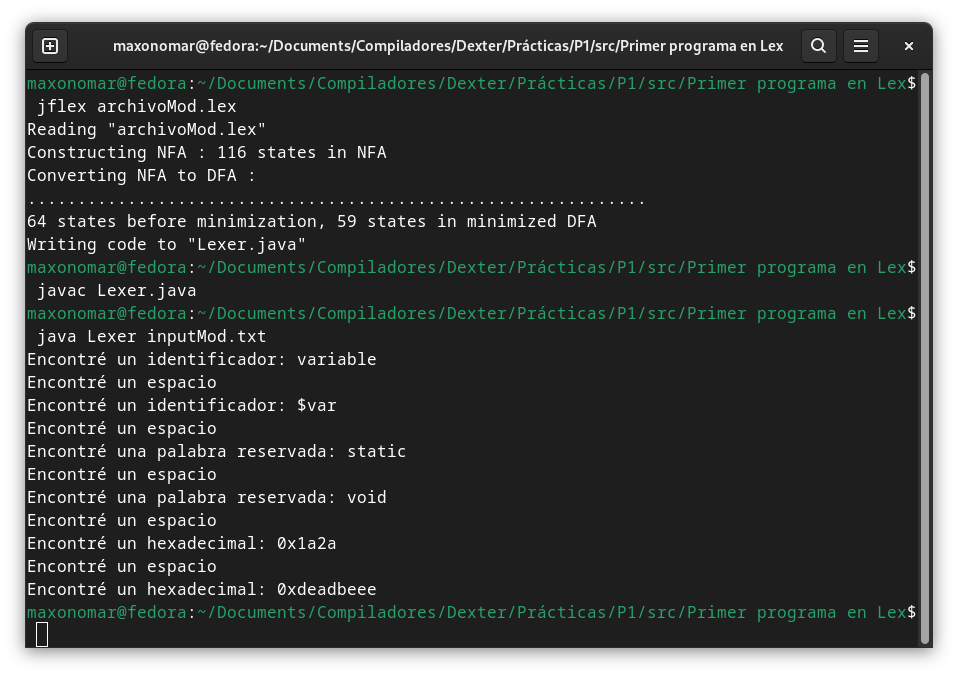
\includegraphics[width=12.5cm]{img/captura}
\centering
\end{figure}

\end{document}
